%======================================================================================
\chapter*{Introdução} \label{cap:intro}
%======================================================================================

\section{Introdução e Justificativa}

A reconstrucão 3D de cenas gerais a partir de múltiplos pontos de vista
usando-se câmeras convencionais, sem aquisição controlada, é um dos grandes
objetivos de pesquisa em visão computacional, ambicioso até mesmo para os dias
de hoje. Aplicações incluem a reconstrução de modelos 3D para uso em
videogames~\cite{Ablan:3DPhoto:book}, filmes~\cite{Ablan:3DPhoto:book},
arqueologia, arquitetura, modelagem 3D urbana (\eg, Google Streetview); técnicas
de \emph{match-moving} em cinematografia para fusão de conteúdo virtual e
filmagem real~\cite{Dobbert:Matchmoving:book}, a organização de uma coleção de
fotografias com relação a uma cena (\eg, o sistema
\emph{Phototourism}~\cite{Argarwal:Snavely:etal:ICCV09} e a funcionalidade
\emph{Look Around} do Google Panoramio e Steet View), manipulação robótica, e a
metrologia a partir de câmeras na indústria automobilística e metal-mecânica.

Os desafios estão ligados às escolhas de grande escala de
representações adequadas e de técnicas que possam modelar simultaneamente com
materiais drásticamente diferentes (\eg, não-Lambertianos), modelos
geométricos (\eg, variedades curvilíneas gerais, descontinuidades, texturas,
deformações, em escalas diferentes), tipos de regiões (com ou sem textura),
condições de iluminação variadas, sombras, fortes diferenças de perspectivas,
desbalanceamento devido a excesso de detalhes em partes menos importantes,
número arbitrário de objetos e câmeras não-calibradas.

Mesmo que um sistema completo esteja fora do alcance da tecnologia atual,
um progresso significativo tem sido atingido nos últimos anos. Por um lado,
uma tecnologia operacional tem evoluido, mais recentemente para sistemas de grande
escala~\cite{Argarwal:Snavely:etal:ICCV09,Pollefeys:VanGool:etal:handheld:IJCV2004},
a partir do desenvolvimento da detecção robusta de
\emph{features}~\cite{mikolajczyk:schmid:IJCV04}, o
\emph{fitting} robusto e seleção de correspondências baseados em \ransac, e o
desenvolvimento de métodos de geometria projetiva para calibrar duas ou três
imagens e progressivamente adicionar imagens e extrair estrutura 3D dessas
\emph{features} na forma de nuvens de pontos. Com o código fonte do sistema
Bundler~\cite{Noah:Bundler,Noah:Steven:Bundler} liberado por Noah Snavely, e sua subsequente incorporação
ao sistema VisualSFM~\cite{Changchang:VisualSFM}, é possível utilizar este sistema para a
reconstrução de patrimônio. 


No paradigma usando-se apenas imagens convencionais -- denominado
\textbf{reconstrução estéreo multiocular passiva} --  a posição das câmeras são
estimadas a partir apenas de imagens, usando pontos de interesse, em seguida uma
nuvem de pontos é reconstruída~\ref{fig:rec3d}.
As câmeras podem então ser utilizadas para obter modelos mais detalhados de reconstrução, como algoritmos de densificação~\cite{Furukawa:Ponce:CVPR2007} e interpolação~\cite{poisson} da nuvem de pontos, bem como demais algoritmos densos de visão estéreo multi-perspectiva/multi-ocular, como os do grupo de Michel Goesele~\cite{Goesele:MVE:2014}, também com código disponível. Tais algoritmos, no entanto, têm problemas, em particular a reconstrução suaviza partes bem-delineadas do objeto, e pode conter buracos em áreas homogêneas. Pode-se, portanto, utilizar a reconstrução 3D de curvas do pesquisador proponente~\cite{Usumezbas:Fabbri:Kimia:ECCV16,Fabbri:Kimia:IJCV2016,Fabbri:Kimia:CVPR10,Fabbri:Giblin:Kimia:ECCV12} para auxiliar na reconstrução mais bem-delinada nesses casos problemáticos, bem como para ajudar
no problema de escalabilidade quando a reconstrução 3D se torna muito grande.
Um segundo paradigma, denominado \textbf{reconstrução estéreo multiocular
ativa}, tem se tornado viável devido à indústria de videogames, e consiste na
utilização de sistemas que alteram o funcionamento de câmeras convencionais,
típicamente usando-se projetores infra-vermelho, laser ou câmeras ToF (time of
flight), como no caso dos dispositivos Kinect, figura~\ref{fig:kinect}.

\begin{figure} [!h]
	\centering
	%   \includegraphics[width=1.0\linewidth]{figs/3d-curve-sketch/system-diagram.eps}
	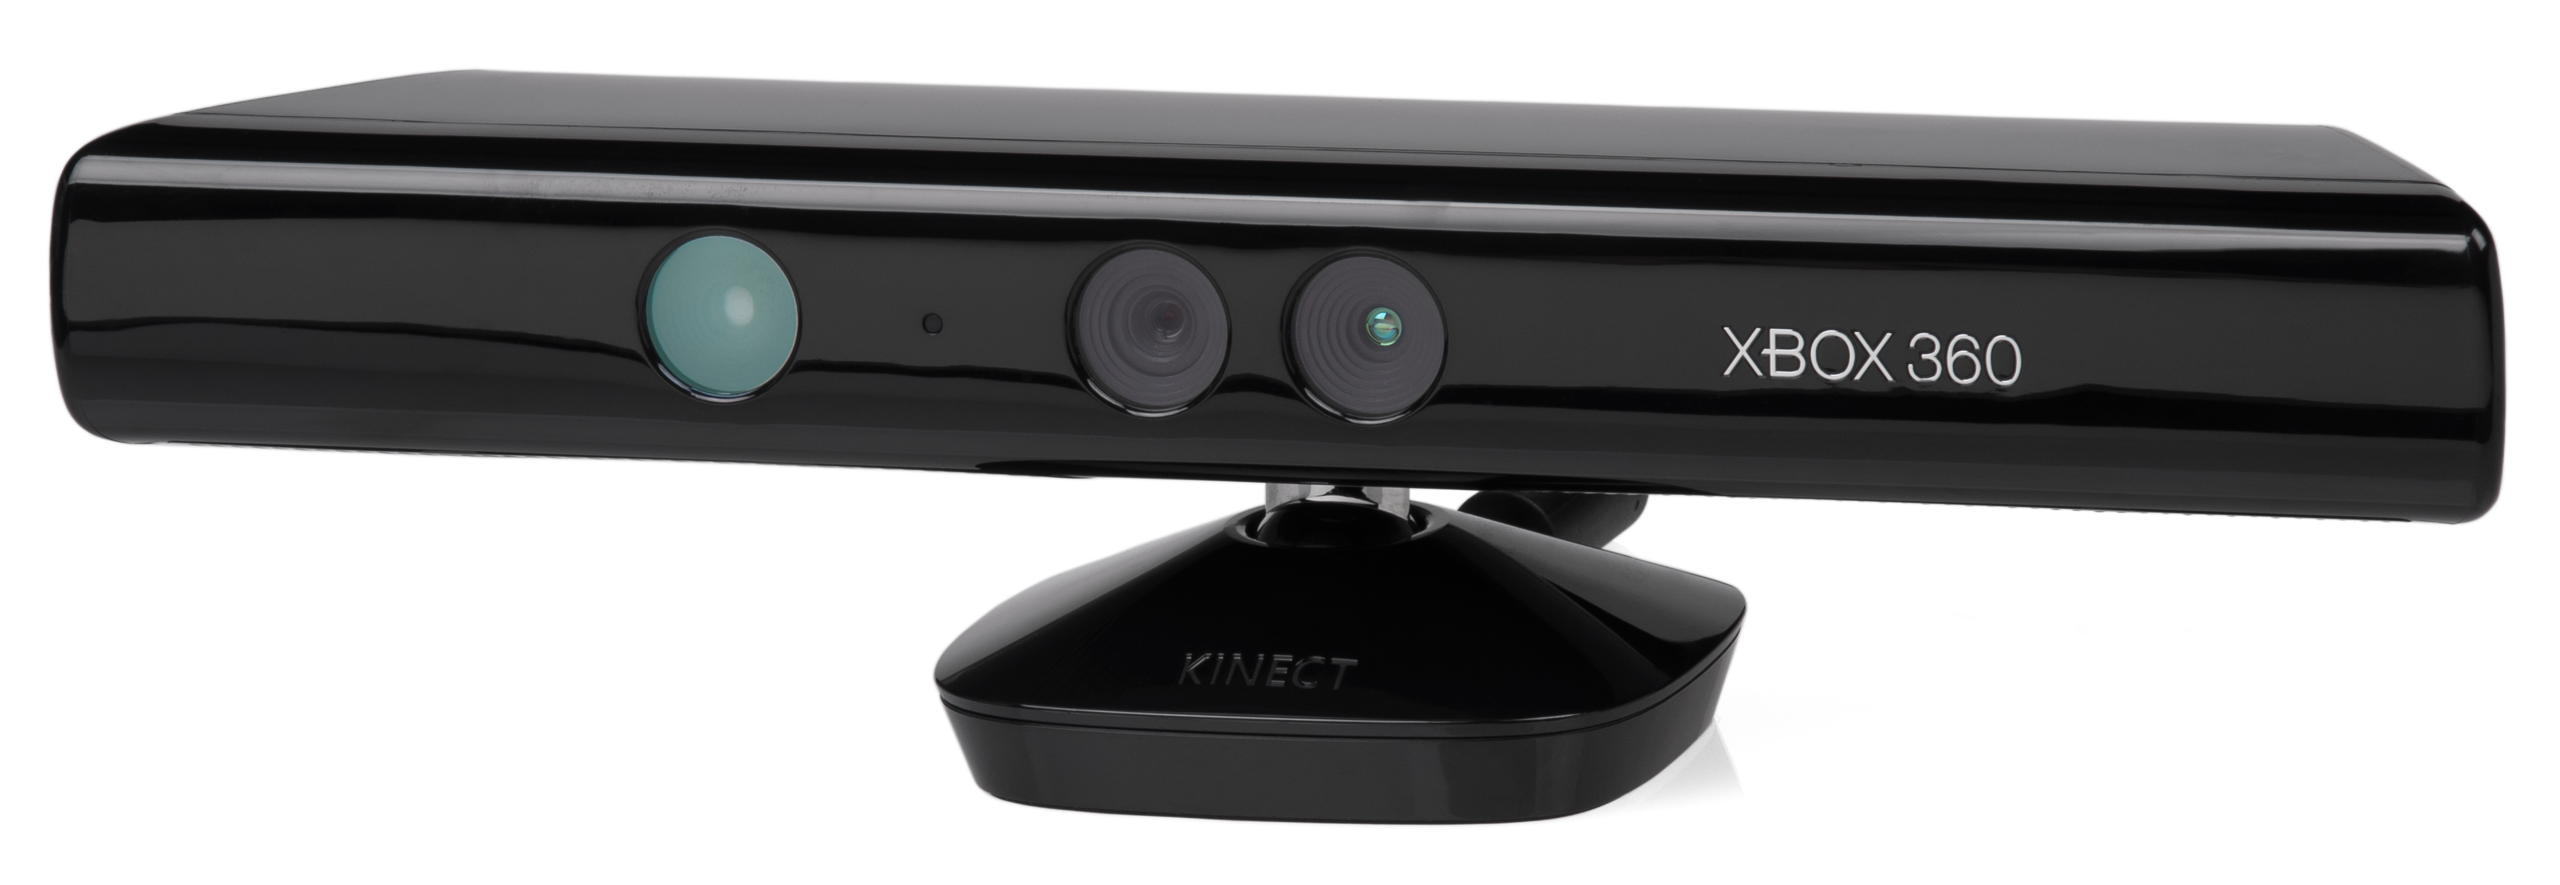
\includegraphics[width=0.45\linewidth]{figs/Xbox-360-Kinect-Standalone.png}(a)
	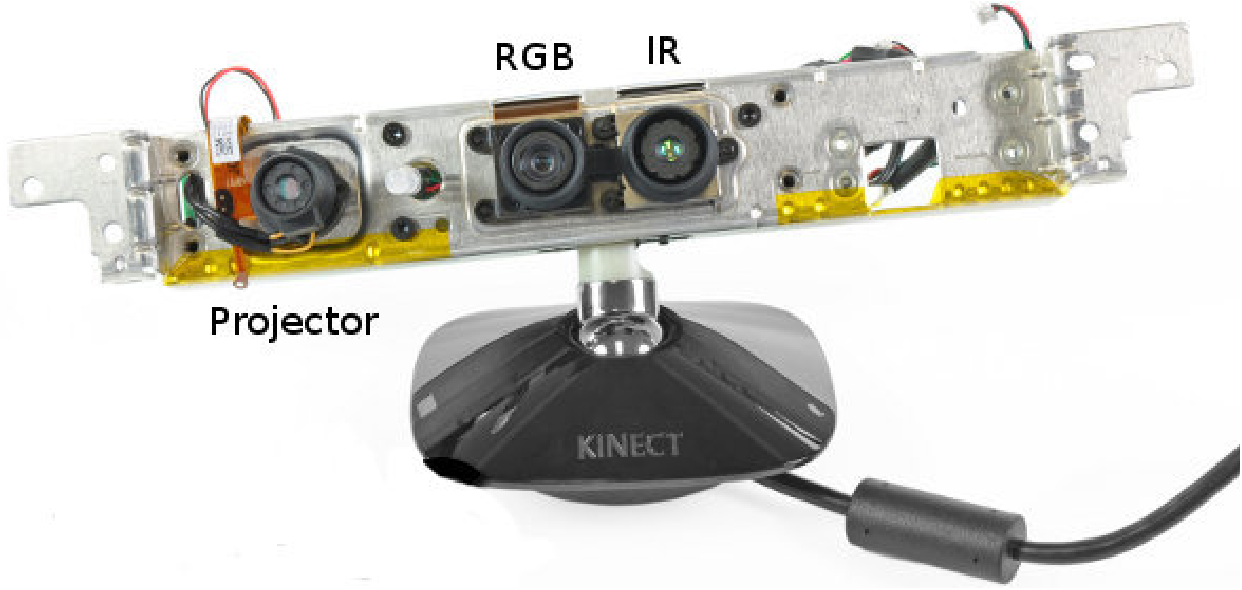
\includegraphics[width=0.45\linewidth]{figs/kinect-internals.pdf}(b)
 	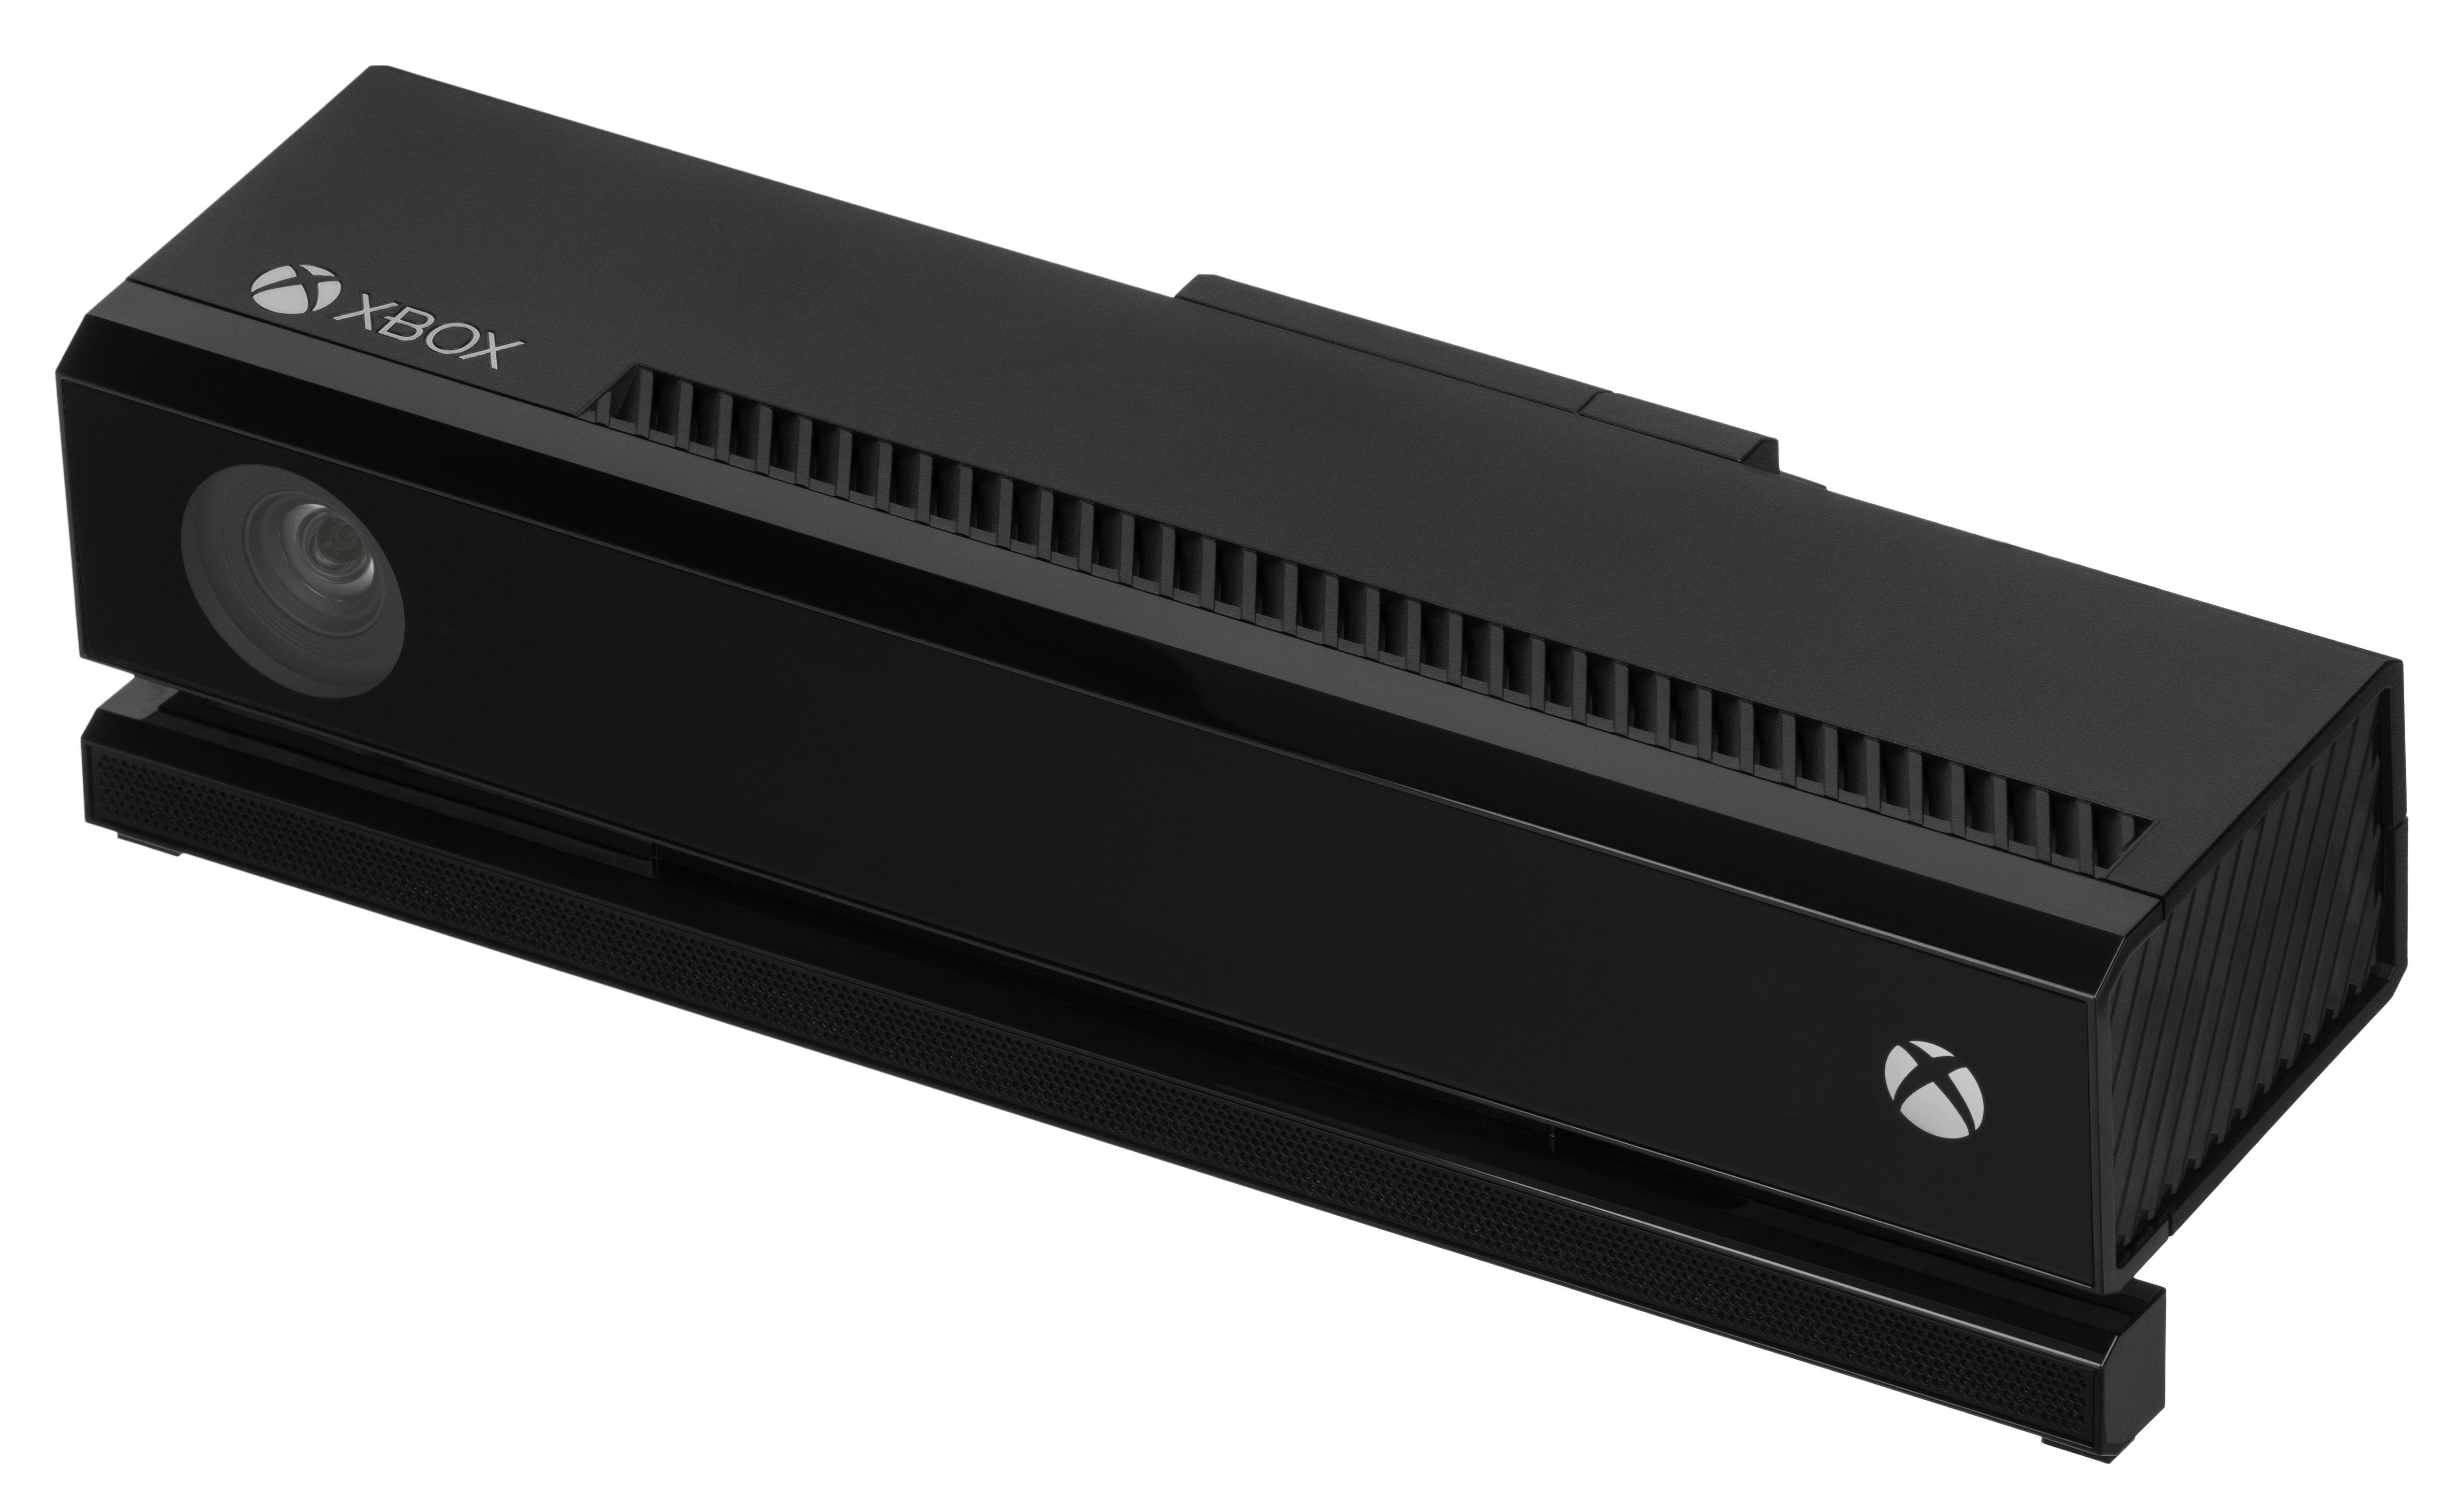
\includegraphics[width=0.45\linewidth]{figs/Xbox-One-Kinect.jpg}(c)
 	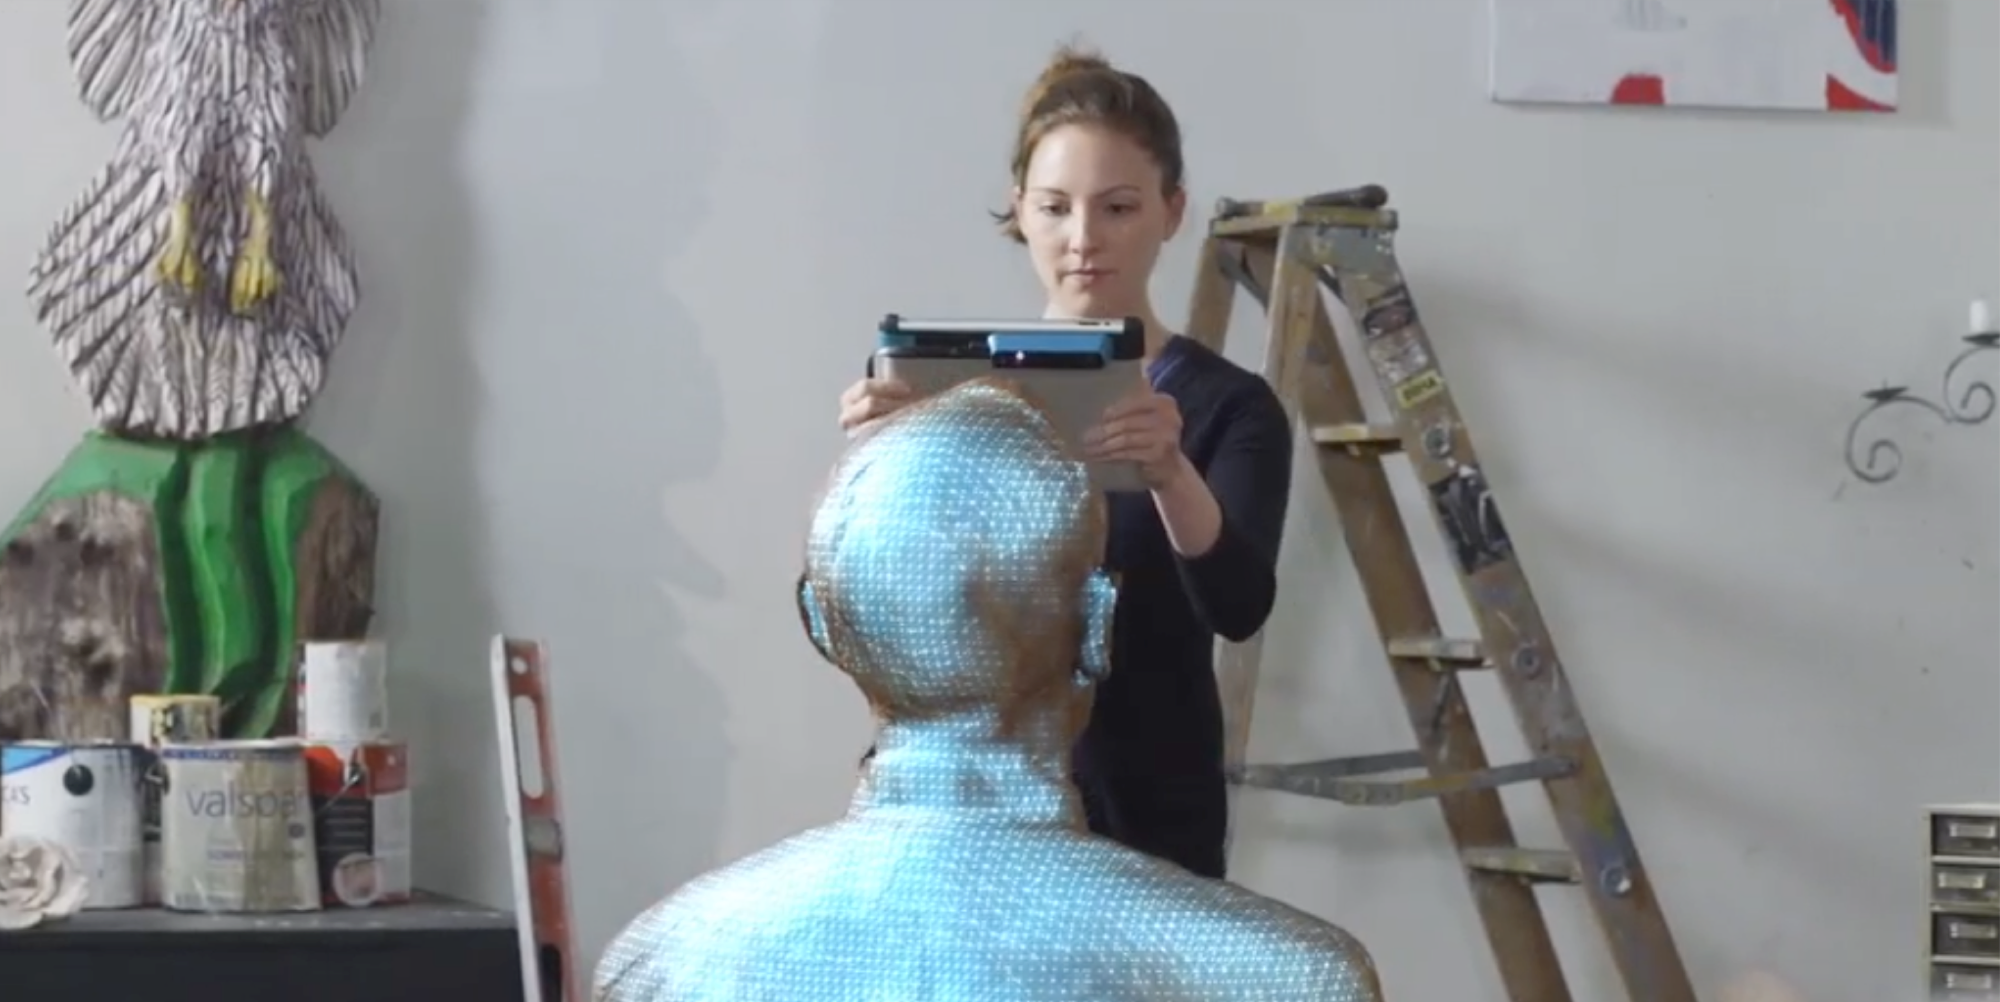
\includegraphics[width=0.45\linewidth]{figs/kinect-handheld1.png} (d)
	\caption{%
   Kinects de primeira geração (a) consistindo de câmeras e projetores
   infra-vermelho (b) e de segunda geração, consistindo de tecnologia ToF (c). 
   Ambos os kinects são largamente utilizados para escaneamento em tempo real, 
   formando a base de scanners manuais (d), porém nem sempre são úteis para 
   preservação detalhada de patrimônio. Um dos objetivos deste
   projeto é explorar os limites desta tecnologia.
	}\label{fig:kinect}
\end{figure}

A preservação de patrimônio tem sido realizada tradicionamente com scanners
dedicados de alto custo, como no projeto David~\ref{fig:david}.
O projeto teve início em 1992 e tem como objetivo a utilização de scanners a laser de profundidade
({\it rangefinder scanners}), aliado com algoritmos que combinam diferentes profundidades e cores da imagem, 
para realizar uma digitalização da parte externa e da superficie de forma acurada da estátua de David 
(porém, esse método pode ser utilizado em diferentes objetos no mundo real, 
como partes de máquinas, artefatos culturais e na indústria de video games, por exemplo). 
Para as partes mais detalhadas, foi utilizado um scanner de menor escala que faz uma pequena 
triangulação com laser de profundidade.

Seria de grande interesse explorar os dois paradigmas supracitados
para avaliar as possibilidades disponíveis no estado da arte de reconstrução 3D
para o escaneamento de baixo custo para a preservação de Patrimônio. O que se
pode atingir com apenas uma filmagem de esculturas realizada por um smartphone,
sem calibração prévia e \emph{in situ}, ou seja, sem ambiente controlado?  Como
esta recontrução se compara nos dias de hoje com a reconstrução realizada por um
scanner padrão baseado em Kinect?

\begin{figure}[!h]
	\centering
	%   \includegraphics[width=1.0\linewidth]{figs/3d-curve-sketch/system-diagram.eps}
	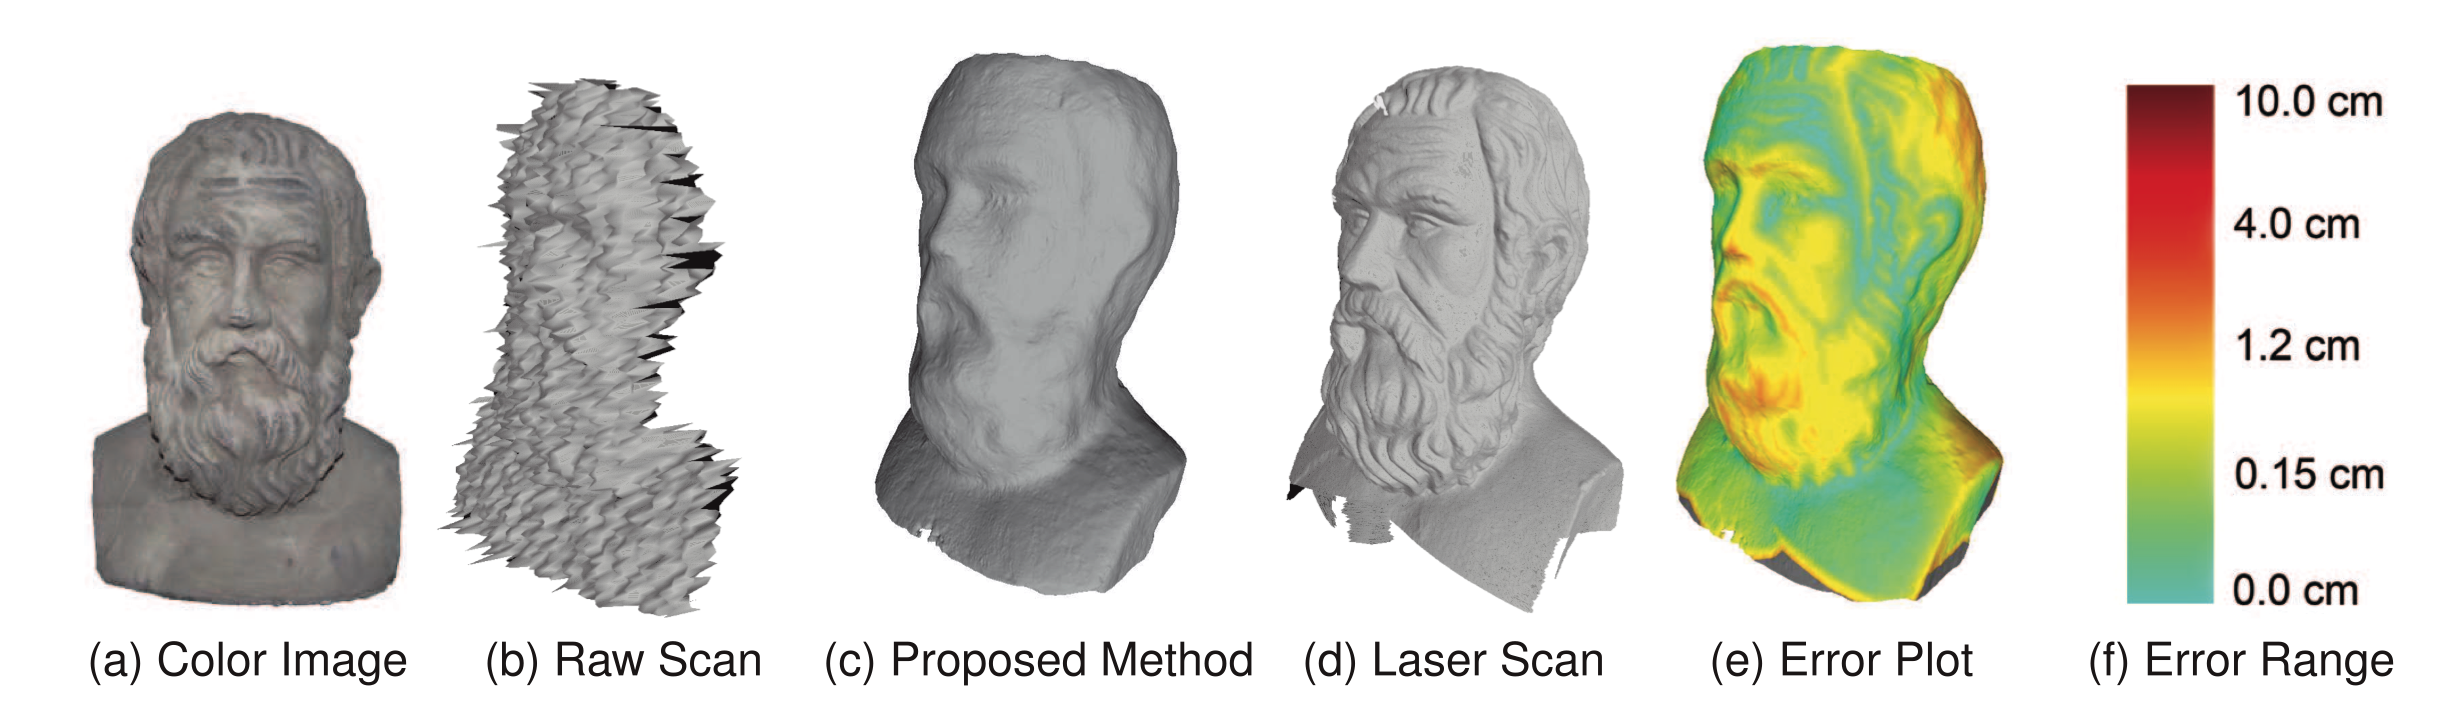
\includegraphics[width=1\linewidth]{figs/kinect-vs-usual.png}
	\caption{%
    A reconstrução usando-se Kinect (de primeira ou segunda geração) usando
    software atual de super-resolução (c) fornece precisão similar a um sistema estéreo de média
    resolução, inferior um sistema a laser de alta qualidade (d) porém de baixo custo e
    muito mais versátil devido ao sistema de aquisição manual e a software
    amplamente utilizado e
    desenvolvido\cite{Cui:Theobalt:etal:PAMI2013,Pajdla:etal:ICCV2011}.
	}\label{fig:rec3d:comparacao}
\end{figure}

\begin{figure}[!h]

\centering

\subfloat[]{\label{fig:davida}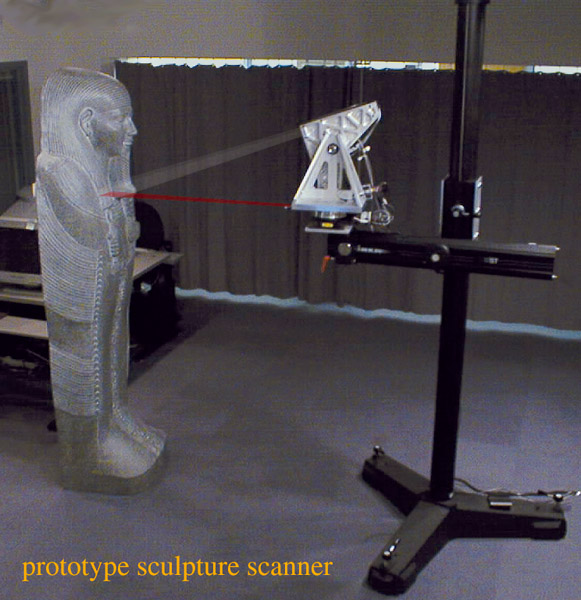
\includegraphics[width=0.18\linewidth]{figs/Proto+Inka+Egypt_light-s.jpg}}
% \vspace{2ex}
\subfloat[]{\label{fig:davidb}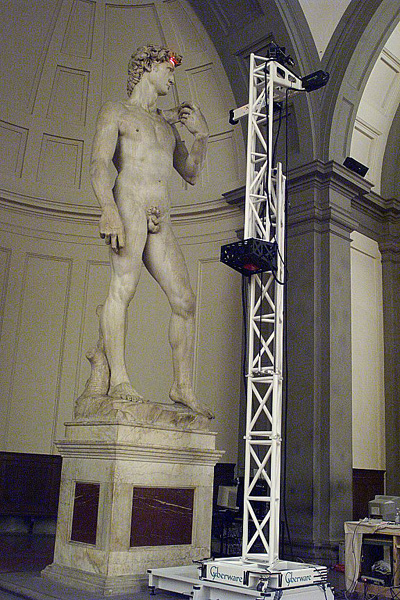
\includegraphics[width=0.18\linewidth]{figs/gantry-with-david-s.jpg}}
\subfloat[]{\label{fig:davidc}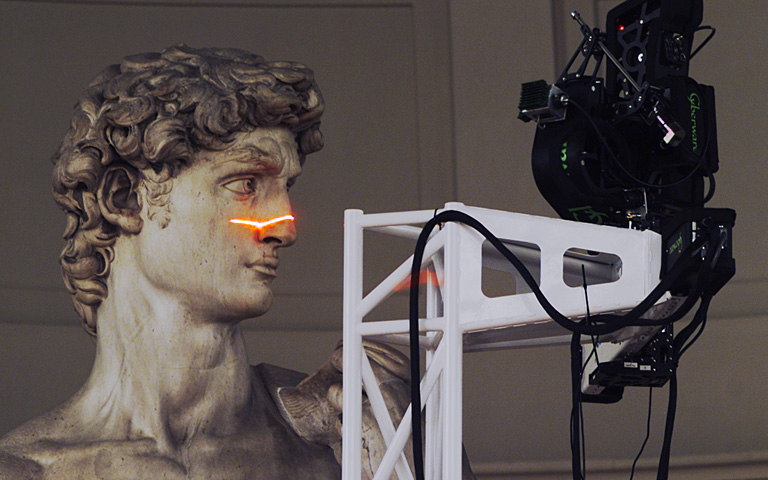
\includegraphics[width=0.18\linewidth]{figs/scanner-head-and-david-head-s.jpg}}
% \vspace{2ex}
\subfloat[]{\label{fig:davidd}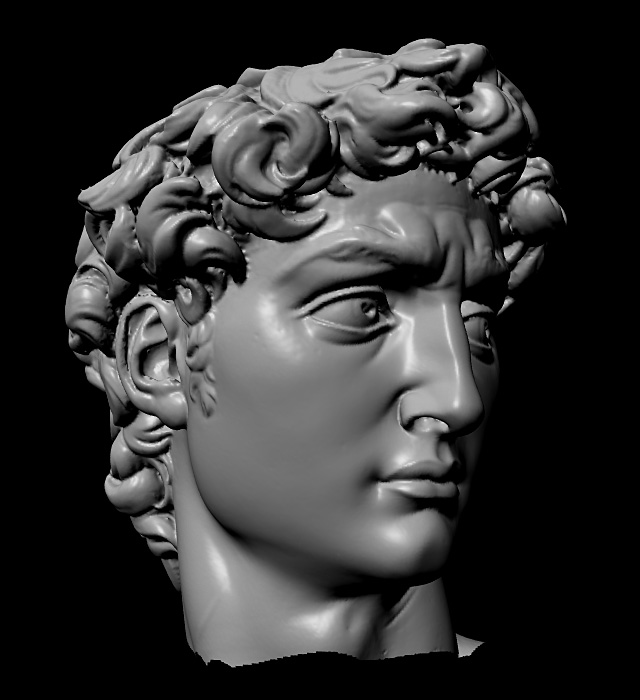
\includegraphics[width=0.18\linewidth]{figs/david-classic-leftlight-s.jpg}}
\caption{%
   Protótipo do scanner a laser de triangulação. O objeto a ser escaneado é uma réplica em tamanho real
   de um sarcófago egípcio (a). O scanner foi reconfigurado para escanear objetos maiores, pois 
   a escultura possui 517 centímetros (b), o da cabeça também sofreu uma reconfiguração, este scanner gira em 90 graus, 
   que faz o laser rotacionar, da posição horizontal para a vertical e também roda em torno da cabeça como um todo (c).
   Para a reconstrucão, o primeiro passo foi alinhar cerca de 100 scans em diversas posicoes, após isso, utilizado um 
   alinhamento automatico em pares dos scans, utilizando um algoritmo modificado de iteracoes de pontos próximos 
   (ICP - \emph {iterated-closest-points}). Após isso, faz-se um processo de relaxação global a fim de minimizar erros 
   de alinhamento por toda a estátua. Depois de alinhados, usa-se o algoritmo de profundidade volumétrica de 
   processamento de imagens (VRIP - \emph {volumetric range image processing} - do Brian Curless) (d).
	}\label{fig:david}
\end{figure}

\subsection{O Jardim do Nêgo, Nova Friburgo}
No caso de Nova Friburgo, há a necessidade redobrada de preservação do
patrimônio, em especial devido às chuvas e deslizamentos inerentes à região.  O
Jardim do Nêgo consiste em grandes esculturas em encostas, cobertas por um tapete de
vegetação, as quais desfrutam de grande reconhecimento regional e internacional~\cite{JardimDoNego:TheGuardian},
figura~\ref{fig:esculturas}.

\begin{figure} [!h]
	\centering
	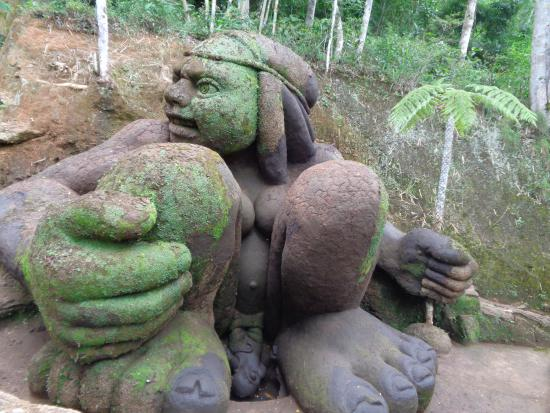
\includegraphics[width=0.3\linewidth]{figs/jardim-do-nego.jpg}
	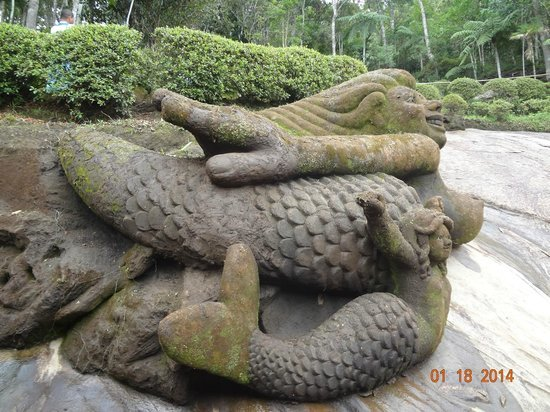
\includegraphics[width=0.3\linewidth]{figs/jardim-do-nego22.jpg}
	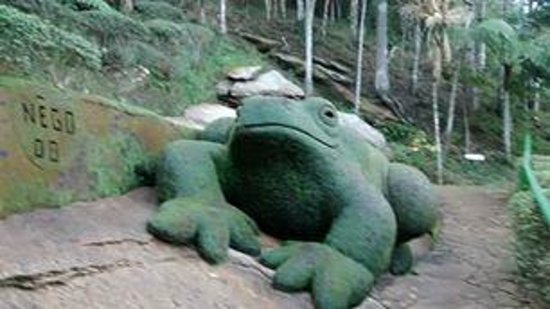
\includegraphics[width=0.35\linewidth]{figs/jardim-do-nego32.jpg}
	\caption{Algumas esculturas do Jardim do Nêgo}\label{fig:esculturas}

\end{figure}


\begin{figure} [!h]
	\centering
	%   \includegraphics[width=1.0\linewidth]{figs/3d-curve-sketch/system-diagram.eps}
	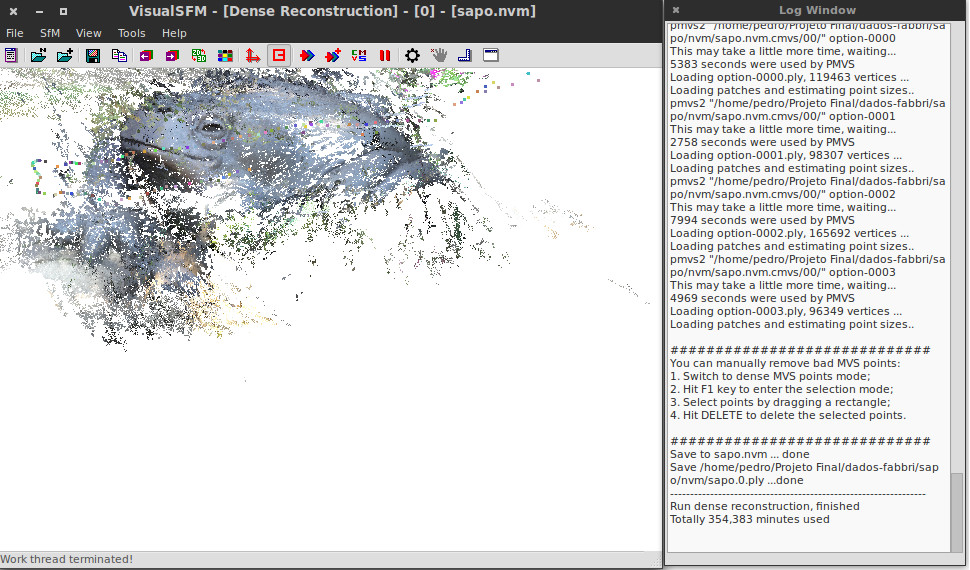
\includegraphics[width=1\linewidth]{figs/rec3d.jpg}
%	\includegraphics[width=0.95\linewidth]{figs/rec3d-curves-pmvs.pdf}
	\label{fig:rec3d}
	\caption{A reconstrução usando-se apenas imagens, sem controle de aquisição, 
	   como em um vídeo de um smartphone filmado em torno do objeto, fornece uma
	   nuvem de pontos, que pode ser
	   densificada~\cite{Noah:Bundler,Noah:Steven:Bundler,Changchang:VisualSFM,Furukawa:Ponce:CVPR2007,Goesele:MVE:2014}, ou
	   atribuída de
	   curvas~\cite{Usumezbas:Fabbri:Kimia:ECCV16,Fabbri:Kimia:IJCV2016,Fabbri:Kimia:CVPR10,Fabbri:Giblin:Kimia:ECCV12}, de forma a preservar a resolução
	   em áreas de alto conteúdo informativo. Tais representações estão sendo
	   atualmente unificadas na pesquisa da área. Este projeto propõe explorar os
	   limites da reconstrução 3D usando-se apenas imagens, no contexto de
	   preservação de patrimônio.}
\end{figure}


Idealizado e criado por Geraldo Simplicio (Nêgo), artista cearense que mora no 
local a mais de 30 anos, ganhou notoriedade por suas esculturas de barro, com traços 
singulares e técnicas únicas. Hoje, trabalha para reconstruir o Jardim da tragédia de 
2011 na região serrana, onde algumas estruturas foram destruídas. Portanto, com o 
consentimento do Nêgo, surgiu a motivação desta pesquisa: além de explorar métodos de 
reconstrucão, também tem o objetivo de eternizar um patrimônio que é reconhecido no mundo
todo.

A preservação das esculturas do Jardim do Nego se torna um desafio à pesquisa em
recontrução 3D, pois apresentam curvas bem delineadas, que são 
representadas de maneira suavizada e empobrecida por métodos convencionais.
Algumas esculturas apresentam pouca textura, quase sem nenhum padrão de textura/musgo.
Seria de grande interesse availiar o potencial de técnicas atuais de
reconstrução 3D geral sem controle de aquisição, as quais têm seu código fonte
disponível na internet.



\section{Objetivos}

O presente projeto pretende fazer com que o aluno ganhe experiência com técnicas
modernas de reconstrução 3D fotogramétrica, no contexto de uma aplicação
bem-definida de preservação de patrimônio. A entrada do sistema deverá ser um
conjunto de vídeos realizados por câmeras de baixo custo, ou um conjunto de
escaneamentos realizados por scanners à mão de baixo custo baseados em Kinect.

O objetivo concreto do aluno será explorar as tecnologias supracitadas para
desenvolver um esquema de escaneamento usando software aberto, câmeras e
scanners de baixo custo, representando o estado da arte em reconstrução 3D sem
restrições de aquisição. Perguntas fundamentais a serem respondidas são: que
nível de detalhe, facilidade e precisão se pode obter usando-se apenas imagens e software
aberto? É possível utilizar scanners de baixo custo baseados em Kinect com
melhorias significativas em termos de qualidade, conveniência ou tempo de
processamento?  Quais são as restrições desses sistemas? Seria útil na prática
uma reconstrução de curvas para auxiliar na reconstrução de nuvem de pontos e de
superfícies densas? Onde o estado da arte deve ser avançado de forma a permitir
uma solução mais conveniente e completa para a preservação de patrimônio?

O principal objetivo em termos de pesquisa científica será comparar as
diferentes abordagens do estado da arte disponíveis para reconstrução 3D e
explicitar suas limitações práticas. O aluno deverá, com o entendimento das
abordagens, desenvolver um esquema de aquisição de esculturas que permita
ampliar os detalhes ou ajudar a resolver os problemas dos métodos. Com a
experiência obtida, o aluno estará pronto para desenvolver pesquisa futura na
área de recontrução 3D, com conhecimento de causa para avaliar direções de
pesquisa de efetivo e alto impacto na prática.




%\section{Curves as a foundation for 3D reconstruction}
%
%In this section we review previous systems for 3D reconstruction, both general
%and specific for water waves. We then motivate the curve-based approach to
%3D reconstruction, camera calibration and general photogrammetry of water waves
%in a number of scenarios. This larger system will use the video tracker proposed
%in the present work as a module and imposes key requirements on its design.
%
%While a fully complete working 3D system addressing all the underlying
%challenges is beyond current technology, significant progress has been made in
%the past few years using approaches that fall into three broad classes,
%depending on whether one focuses on correlating isolated points, surface
%patches, or curvilinear structures across views, as described below.
%
%A vast majority of multiview reconstruction methods rely on correlating isolated
%interest points across views to produce an unorganized 3D cloud of points.  The
%\textbf{interest-point-based approach} has been highly successful in
%reconstructing large-scale scenes with {\em texture-rich images}, in systems
%such as in Phototourism and recent large-scale 3D reconstuction
%work~\cite{Heinly:Frahm:etal:CVPR2015,Pollefeys:VanGool:etal:handheld:IJCV2004,Argarwal:Snavely:etal:ICCV09,Diskin:Vijayan:JEI2015}.
%Despite their usefulness, these methods generally cannot represent smooth,
%textureless regions (due to the sparsity of interest points in image regions
%with homogeneous appearance), or regions that change appearance drastically
%across views. 
%%%% TODO put somewhere else, its out of place but important:
%%even though contours clearly match. \indraftnote{Ben: we shouldn't change the
%%previous sentence since it was to attend a reviewer criticism on our ECCV
%%paper}
%This limits their applicability, especially in man-made
%environments~\cite{Simoes:etal:SVR2014} and objects such as
%cars~\cite{Shinozuka:Saito:VRIC14}, non-Lambertian surfaces such as that of the
%sea (as in the case of the present work), appearance variation due to changing
%weather~\cite{Baatz:Pollefeys:etal:ECCV12} (as is also the case of the open sea), and wide
%baseline~\cite{Moreels:Perona:IJCV07} (as is also the case in the present work).
%% TODO: update info with lofting paper and IJCV
%
%\todo{fig with 3D curve-based rec as motivation}
%
%Another approach matches intensity patterns across views using multiview stereo,
%producing denser point clouds or mesh reconstructions.  \textbf{Dense multi-view
%stereo} produces detailed 3D reconstructions of objects imaged under controlled
%conditions by a large number of precisely calibrated
%cameras~\cite{Furukawa:Ponce:CVPR2007,Habbecke:Kobbelt:CVPR2007,Hernandez:Schmitt:CVIU04,Goesele:etal:ICCV07,Seitz:etal:CVPR06,Calakli:etal:3DIMPVT2012,Restrepo:etal:JPRS2014}.
%For general, complex scenes with various kinds of objects and surface
%properties, this approach has shown most promise towards obtaining an accurate
%and dense 3D model of a given scene.  Homogeneous areas, such as walls of a
%corridor, repeated texture, and areas with view-dependent intensities create
%challenges for these methods.  All of these challenges are present on the water surface.
%
%A smaller number of techniques correlate
%and reconstruct image \textbf{curvilinear structure} across views, resulting in 3D curvilinear 
%structure. Pipelines based on straight
%lines (see~\cite{Lebeda:etal:ACCV2014,Zhang:line:PHDThesis2013,Fathi:etal:AEI2015} for recent reviews),
%algebraic and general curve features~\cite{Teney:Piater:3DIMPVT12,Litvinov:etal:IC3D2012,Fabbri:Kimia:CVPR10,Fabbri:Giblin:Kimia:ECCV12,Wendel:etal:CVWW2011,Berthilsson:etal:IJCV2001,Fabbri:Kimia:EMMCVPR2005}
%have been proposed, but some lack generality, \eg, requiring 
%specific curve models~\cite{Carrasco:etal:LNCS2012}.
%The 3D Curve Sketch
%system~\cite{Fabbri:PHD:2010,Fabbri:Kimia:CVPR10}
%and the 3D drawing
%system~\cite{Usumezbas:Fabbri:Kimia:ECCV16,Usumezbas:Fabbri:Kimia:CVPR17,Fabbri:Kimia:CVPR16}
%are the state of the art in curve reconstruction for arbitrary geometry. It is
%the suitability to this system that we aim for in the present work.
%See also~\cite{Fabbri:Giblin:Kimia:ECCV12,Fabbri:Kimia:IJCV2016,Fabbri:Kimia:EMMCVPR2005}.
%
%\todo{semantics: why would we want to separate reflects vs clean wave signal}
%%Many applications such as robotics~\cite{Carlson:etal:ICRA2014}, urban planning
%%and industrial design~\cite{Yee:architectural:book,Leggitt:drawing:book},
%%Figure~\ref{fig:architectural:drawing}, require a structured 3D
%%representation which makes explicit 3D curves and 3D surfaces; spatial
%%relationships among curves, among surfaces and between curves and surfaces;
%%3D components which make possible semantic interpretations of these structures,
%%\eg, building ridges, building faces, chimneys, etc. The previous approaches
%%have focused on surface representation as a cloud of points or as meshes, but
%%not as much work has focused on representing general 3D curves.  This is a
%%significant shortcoming because objects in the world are typically annotated %by 3D curves such as ridges,
%%reflectance boundaries, and texture boundaries.
%
%%While these approaches have been widely successful in some applications,
%%there has been a real demand for a complementary approach that produces more
%%\emph{structured}, efficient and recognizable 3D reconstructions beyond point
%%clouds, meshes and voxel volumes, that scales to more general assumptions as
%%demanded by applications such as robotics~\cite{Carlson:etal:ICRA2014} and urban
%%planning/industrial design, Figure~\ref{fig:architectural:drawing}.
%%
%% COOL but ben removed:
%%(\ie, more structured and recognizable than point clouds, while lighter more
%%condensed than 3D meshes or voxel volumes for large-scale scenes) 
%%
%%This paper proposes a novel multiple view stereo
%%system based on image curve content to address this demand, producing
%%condensed, structured and integrated representation of general real-world 3D scenes as
%%graphs of linked 3D contour fragments, which we refer to as the \emph{3D Curve Drawing} of a
%%scene. 
%
%The plethora of multiview representations, as documented above, arise because 3D
%structures are geometrically and semantically
%rich~\cite{Zia:Stark:Schindler:IJCV2015,Feng:Medioni:etal:SIGGRAPH14}.  A
%building, for example, has walls, windows, doorways, roof, chimneys, etc. The
%structure can be represented by sample points (\ie, unorganized
%cloud of points) or a surface mesh where connectivity among points is captured.
%This representation, especially when rendered with surface albedo or texture, is
%visually appealing. However, the representation also leaves out a great deal of
%semantic information: which points or mesh areas represent a window or a wall?
%Which two walls are adjacent? The representation of such components, or parts,
%requires an explicit representation of part boundaries such as ridges, as well
%as where these boundaries come together, such as junctions.
%
%The same point can equally arise if objects in the scene were solely defined
%by their curve structures. A representation of a building by its ridges may
%usually give an appealing impression of its structure, but it fails to identify
%the walls, \ie, which collection of 3D curves bound a wall and what its geometry
%is. Both surfaces and curves are important and needed, \eg, in
%applications such as robotics~\cite{Carlson:etal:ICRA2014}, urban planning and
%industrial design~\cite{Yee:architectural:book,Leggitt:drawing:book}, Fig.~\ref{fig:architectural:drawing}.
%Note, however, that water images are also challenging in this sense, since there
%are usually no well-defined semantics or curve topology, as the patterns in
%water can vary wildly -- there is no fixed structure or topology on its patterns.
%
%The ultimate goal of the tracker presented in this work as a module for a larger system 
%to produce a 3D curve-based reconstruction, augmented with the recovery of
%surfaces (when there is enough data) so that 3D curves bound the 3D curve
%segments. The 3D curve reconstruction can also be of independent value in applications
%such as fast recognition of general 3D scenery~\cite{Wendel:etal:CVWW2011},
%efficient transmission of general 3D scenes, scene understanding and modeling by
%reasoning at junctions~\cite{Mattingly:etal:JVLC2015}, consistent
%non-photorealistic rendering from video~\cite{Chen:Klette:IVT2014}, modeling of
%branching structures, among
%others~\cite{Rao:etal:IROS2012,Kowdle:etal:ECCV10,Ruizhe:Medioni:CVPR2014}.
%
%In general, image curve fragments are attractive because they have
%good localization, they have greater invariance than interest points to changes
%in illumination, are stable over a greater range of stereo baselines, and are typically
%denser than interest points.  Furthermore, the reflectance or ridge curves
%provide boundary condition for surface reconstruction, while occluding contour
%variations across views lead to surfaces~\cite{Giblin:Motion:Book,Liu:Cooper:etal:PAMI07,Crispell:etal:LNCS2009}.
%Recent studies strongly support the notion that image curves contain much of the
%image
%information~\cite{Koenderink:Wagemans:etal:iPerception2013,Zucker:PIEEE2014,Kunsberg:Zucker:LNM2014,Cole:etal:SIGGRAPH09}.
%Moreover, curves are structurally rich as reflected by their differential
%geometry, a fact which is exploited both in recent computer
%systems~\cite{Zucker:PIEEE2014,Abuhashim:Sukkarieh:IROS2012,Fabbri:Giblin:Kimia:ECCV12,Fabbri:Kimia:CVPR10}
%and peception studies~\cite{Fleming:etal:PNAS2011,Zucker:PIEEE2014}.
%\todo{dayany: pode usar figuras deste paragrafo que estao na minha tese, para
%melhora-lo na sua dissertacao}

%\section*{Configuração de aquisição}\label{sec:setup}
%Uma vez que a configuração da nossa aquisição de dados é central para todo este
%trabalho, agora o apresentamos com mais detalhes.
%
%As dimensões do tanque de onda multidirecional na COPPE/UFRJ são mostradas na
%Figure~\ref{fig:tank:dims}:
%ele tem $45m$ de comprimento e $30m$ de largura; a profundidade é de $15m$, com um poço
%central com $10m$ adicionais localizados a $20m$ de distância do gerador de
%ondas. Tem duas praias absorventes, uma localizada no final de seu comprimento e
%outra em um dos lados.
%
%No conjunto de dados tratado neste trabalho, o tanque gerou ondas monocromáticas
%regulares filmadas a partir de quatro direções diferentes. Cada vídeo tem
%duração de 3min, resolução 1920x1080 e 30 fps, cerca de 300MB cada. As quatro
%câmeras sincronizadas são duas cabeças estéreo de pequena distância, espaçadas 45
%graus entre si, Figura~\ref{fig:4views}. As cabeças estéreo estão em disparidade vertical.
%Recomendamos fortemente ao leitor que assista os vídeos nos materiais
%complementares deste manuscrito.
%
%Além das câmeras, existem sondas que medem as ondas em um único ponto, que podem
%ser usadas em trabalhos futuros para fins de validação.
%
%\begin{figure}
%  \caption{Dimensões do tanque na nossa configuração.}
%  \centering
%  \includegraphics[width=\linewidth]{figs/wavetank-dims.pdf}
%  \source{O autor, 2017.}
%  \label{fig:tank:dims}
%  \ReduceAfterCaptionfigspace
%\end{figure}
%\todo{fig with camera placement}

%\section{Previous techniques on the photogrammetry of water waves}
%Measuring patterns on the surface of the water from images presents all the
%aforementioned challenges to general computer vision techniques. Specialized
%techniques have achived success in certain configurations that minimize some of
%these challenges, but may not generalize well to more challenging conditions.
%As we will see, these techniques assume some of the following restrictions:
%
%\begin{itemize}
%  \item A sea state that has enough texture, \eg, choppy and not very smooth.
%  \item A surface geometry that is not fully 3D, called 2.5D in computer vision.
%    One consquence is that these systems cannot cope with self-occlusion, which
%    is particularly useful when tracking wave crests or filming from a slant
%    angle.
%  \item Illumination conditions must be such that the water surface is mostly
%    diffuse, as to be well-modeled by a lambertian illumination model. This
%    means these approaches will either have holes or interpolate through
%    unreliable measurements.
%\end{itemize}
%All of these restrictions can be dealt with by the use of curve-based features, as done
%in the present work. We now briefly review some of the recent techniques that are most widely
%used in the field of ocean engineering and physical oceanography.
%
%\paragraph{Optical flow techniques.} Certain techniques attempt to examine
%optical flow and similar information of deformation patterns in the water surface from a single
%video~\cite{Rapizo:etal:JCR2015}.
%The conditions have to be designed such the brighness-constancy condition of
%optical flow and other assumptions can be employed. The disadvantages of these
%techniques is that the wave information from a single video from a single
%viewpoint is highly ambiguous, leading to rigid, highly specialized solutions
%(with strong pre-calibration and assumptions on acquisition conditions). The understanding
%of a single view-video is, however, simple for certan scenarios, and can be very
%useful when our proposed four-view system performs spatio-temporal reasoning. 
%
%An early work by Amorim~\etal~\cite{Amorim:Fabbri:etal:IRCE2013} explored how
%the dynamics of the sea state at beaches can be predicted and represented by
%unsupervised machine-learning through diffusion maps from single videos. This
%works presents useful ideas on how machine learning can be used later on the
%proposed system, to update the model and to compress the video based on
%previously seen data.
%

%\paragraph{Técnicas existentes de visão estéreo.} 
%O objetivo deste trabalho é produzir entrada para sistemas de reconstrução 3D.
%Os sistemas
%existentes~\cite{Benetazzo:CE2006,Benetazzo:CE2012,Gallego:etal:TGRS201,Fedele:etal:OM2013,Fedele:etal:MCS2012,Benetazzo:etal:CE2016,Gallego:etal:TIP2013,Bergamasco:etal:CG2016}
%não são capazes de reconstruir as imagens na configuração proposta, portanto
%exploramos técnicas baseadas em curvas. Veja
%Figura~\ref{fig:benetazzo:variational} para um exemplo.

%The main idea is to represent the surface to be reconstructed as a single
%function $z = f(x,y)$, which is what is called 2.5D surface in computer vision.
%This surface is defined on a region of interest (ROI), and optimized using two
%techniques. The first technique is based on traditional dense stereo that assume
%a Lambertian surface, with pixel regions to be matched along epipolar lines. The
%second technique is to optimize the surface using variational methods, with
%smoothness and data-fidelity terms. Both techniques produce results similar to
%the one illustrated in Figure~\ref{fig:benetazzo:variational}.
%
%As discussed later in the present text, Figure~\ref{fig:roigamma}
%and~\ref{fig:3o:zoom}, these techniques are not adequate for our
%dataset as they suffer from all three aforementioned challenges. For our
%dataset, there may be very low texture away from wave crests, so that there is
%no reliable information at large smooth regions. In these cases, for $(x,y)$ in
%smooth regions, the variational approaches may optimize spurious $z=f(x,y)$
%values. Our curve-based approach, on the other hand, focuses processing where
%the reliable information is, \ie, the wave curves. 
%
%\todo{there are nicer 3D images out there}
%\begin{figure}
%  \caption{As técnicas estéreo mais usadas na literatura só modelam ondas
%    curtas e não modelam geometria 3D complexa, o que pode ser feito com
%    curvas.} 
%  \centering
%  \includegraphics[width=\linewidth]{figs/benetazzo-process-variational.png}
%  \source{~\cite{Gallego:etal:TGRS201,Gallego:etal:TIP2013}}
%  \label{fig:benetazzo:variational}
%  \ReduceAfterCaptionfigspace 
%\end{figure} %\todo{fig with camera placement}

\section{Organização deste manuscrito}

O trabalho foi estruturado da seguinte maneira: previamente introduzimos os métodos baseados em pontos de interesse no Capítulo~\ref{sec:pontosdeinteresse}, destacando suas funcionalidades. No Capítulo~\ref{sec:denserecon} discutimos e aprofundamos o  funcionamento de cada algoritmo de reconstrução densa empregados, apresentando e debatendo, comparativamente, pontos à favor e contra; O Capítulo~\ref{sec:kinect} é apresentada a técnica de reconstrução utilizada nos  {\it Kinects}, da Microsoft; Com isso, temos o  Capítulo~\ref{sec:visualsfm}, que é dedicado à ferramenta gráfica utilizada para a obtenção dos resultados (VisualSfM) dos algoritmos de reconstrução densa utilizados. Finalmente, apresentamos os resultados e conclusões do trabalho, bem como sugestões para implementações e trabalhos futuros.
%Este trabalho está organizado da seguinte forma: discutimos as técnicas de
%extração de curva sem aprendizagem de máquina supervisionada no
%Capítulo~\ref{sec:cfrag:extraction}. No Capítulo~\ref{sec:learning:chapter},
%discutimos maneiras pelas quais essas técnicas podem ser melhoradas
%usando dados de treinamento anotados por humanos como entrada para uma
%aprendizagem de máquina geométrica de topologia e semântica de fragmentos de
%curva. A maior parte deste material é
%de~\cite{Guo:etal:CVPR14,Guo:etal:PAMI2017:submitted,Tamrakar:PHD:2008}, com esclarecimentos
%substanciais e comentários sobre as questões relativas aos nossos objetivos
%específicos. No Capítulo~\ref{sec:generic:datasets}, apresentamos o processo de
%captura de dados confiáveis (\emph{ground-truth}), comparando os conjuntos de dados anteriores com o problema proposto
%neste trabalho para a água. Nos capítulos restantes, apresentamos e discutimos
%nossos resultados para vários vídeos em tanques de água. Partes deste trabalho
%foram apresentadas em~\cite{Fabbri:WaterWaves2016,Fabbri:WaterWaves2017,Souza:Fabbri:WaterWaves2017}.

%======================================================================================
